\begin{frame}{Example: Blackhole Freedom}
    Property: each packet should reach $b$
    \begin{center}
        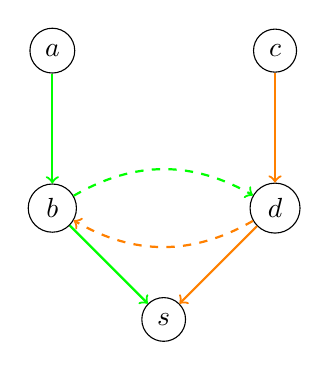
\begin{tikzpicture}[
                node distance={20mm},
                main/.style = {draw, circle},
                s/.style = {->,thick},
                d/.style = {->,thick,dashed} ]
            \node[main] (s) {$s$};
            \node[main] (b) [above left of=s] {$b$};
            \node[main] (a) [above of=b] {$a$};
            \node[main] (d) [above right of=s] {$d$};
            \node[main] (c) [above of=d] {$c$};
            \draw[thick,green,->] (a) -- (b);
            \draw[thick,green,->] (b) -- (s);
            \draw[thick,green,->,dashed] (b) edge[bend left] (d);
            \draw[thick,orange,->] (c) -- (d);
            \draw[thick,orange,->] (d) -- (s);
            \draw[thick,orange,->,dashed] (d) edge[bend left] (b);
        \end{tikzpicture}
    \end{center}
    \begin{equation*}
        \begin{aligned}[c]
            P   & = p!1                             \\
            Q   & = q!1                             \\
            N   & = F \oplus p?1;N_p \oplus q?1;N_q \\
            N_p & = F \oplus q?1;N_{pq}           \\
            N_q & = F \oplus p?1;N_{pq}           
        \end{aligned}
        \qquad\qquad
        \begin{aligned}[c]
            F   & = as \oplus cs                    \\
            F_{pq}      & = ab \vee cd  \\
            SDN         & = \delta_{\mathcal{L}} (N
            \parallel P \parallel Q)                \\
            \mathcal{L} & = \s{p!1,p?1,q?1,q?1}     
        \end{aligned}
    \end{equation*}
\end{frame}

\begin{frame}{Example: Blacklist}
    \begin{align*}
        E  = \s{ &
        p_1,p_2,q_1,q_2,p',q',ab_1,ab_2,ab_3, ac_1,ac_2,     \\
                 & ac_3,ad_1,ad_2,cb_1,cb_2,cd_1,cd_2,cd_3 }
    \end{align*}
    We encode the property as:
    \begin{align*}
        \f{PV} & = \forall c \in \mathcal{F}(ES),
        \forall e \in c. l(e) =  \alpha\cdot\pi \Rightarrow \pi(sw) = s
    \end{align*}
    \begin{center}
        \begin{tikzpicture}[scale=0.8]
            \crd{0}{0}{$\emptyset$}
            \crd[left]{-2}{1}{$\s{p_1}$}
            \crd[left]{-2}{2}{$\s{p_1,q_1}$}
            \crd[left]{-2}{3}{$\s{p_1,q_1,ad_1}$}
            \crd[right]{2}{1}{$\s{q_2}$}
            \crd[right]{2}{2}{$\s{p_2,q_2}$}
            \crd[right]{2}{3}{$\s{p_2,q_2,ad_2}$}
            \draw [ultra thick] (-2,1) -- (-2,2);
            \draw [ultra thick] (-2,2) -- (-2,3);
            \draw [ultra thick] (0,0) -- (2,1);
            \draw [ultra thick] (0,0) -- (-2,1);
            \draw [ultra thick] (2,1) -- (2,2);
            \draw [ultra thick] (2,1) -- (2,3);
        \end{tikzpicture}
    \end{center}
\end{frame}

\begin{frame}{Example: Blacklist}
    We can define $C(p_1,q_1) = \F$ as an actual cause of $PV$
    using the witness $(C(p_2,q_2),\T,\T)$
    \begin{center}
        \begin{tikzpicture}
            \crd{0}{0}{$\emptyset$}
            \crd[left]{-2}{1}{$\s{p_1}$}
            \crd[left]{-2}{2}{$\s{p_1,q_1}$}
            \crd[above]{-1}{3}{$\s{p_1,q_1,ab_1}$}
            \crd[left]{-3}{3}{$\s{p_1,q_1,cd_1}$}
            \crd[right]{2}{1}{$\s{q_2}$}
            \crd[right]{2}{2}{$\s{p_2,q_2}$}
            \crd[above]{1}{3}{$\s{p_2,q_2,ab_2}$}
            \crd[right]{3}{3}{$\s{p_2,q_2,cd_2}$}
            \draw [ultra thick] (-2,1) -- (-2,2);
            \draw [ultra thick] (-2,2) -- (-1,3);
            \draw [ultra thick] (-2,2) -- (-3,3);
            \draw [ultra thick] (0,0) -- (2,1);
            \draw [ultra thick] (0,0) -- (-2,1);
            \draw [ultra thick] (2,1) -- (2,2);
            \draw [ultra thick] (2,2) -- (1,3);
            \draw [ultra thick] (2,2) -- (3,3);
        \end{tikzpicture}
    \end{center}
\end{frame}